\chapter{Grundlagen Netzwerk}
In diesem Kapitel werden die Grundlagen von AMIDAR und der für diese Arbeit genutzten Netzwerkprotokolle erläutert. 

\section{Netzwerk Schichtenmodell}
Die Netzwerk-Kommunikation zwischen Anwendungen wird üblicherweise als Schichtenmodell beschrieben.  
Die unterste Schicht stellt dabei das \textit{Physical Layer} dar und beschreibt die physische Übertragung von Daten. 
Darüber sorgt die Sicherungsschicht für eine funktionierende Verbindung zwischen den Endgeräten und dem Übertragungsmedium. Auf dieser Schicht wird zum Beispiel das Ethernet Protokoll eingesetzt, das Netzwerkteilnehmer über die MAC-Adresse im lokalen Netz adressiert, die übertragenen Daten auf Fehler überprüft und im Zweifel verwirft. 
Darüber kommt die Vermittlungsschicht, in der die Endgeräte über mehrere Subnetze hinweg adressiert werden und Routing und Datenflusskontrolle gesteuert werden. Ein wichtiges Protokoll dieser Schicht ist das IP Protokoll. \\
Bei einer Datenübertragung von einer Anwendung zu einer auf einem anderen Endgerät laufenden, werden die Daten durch die Schichten nach unten gereicht, wobei in jeder Schicht ein neuer Header erzeugt wird, der für die jeweilige Schicht wichtige Informationen enthält. Zum Beispiel werden die Daten von der Anwendung mit betriebssystemabhängigen Systemaufrufen an den TCP-Stack übergeben. Dieser erzeugt ein TCP-Paket, das außer den Daten einen Header enthält, welcher Informationen bereitstellt, die sowohl für das richtige Zusammensetzen der einzelnen Datenpakete beim Empfänger, als auch für die Zuordnung der übertragenen Daten zu der jeweiligen Anwendung benötigt werden.\\\\
Bei der anschließenden Erzeugung des IP-Pakets bildet das TCP-Paket, bestehend aus Nutzdaten und TCP-Header, die zu übertragenden Daten. Der IP Header enthält unter anderem die IP-Adressen des Ziel- und Quell-Geräts. Das IP Paket bleibt im Normalfall unverändert, bis das Zielgerät erreicht ist. An der nächst unteren Ebene steht das Ethernet Datagramm. Es enthält neben dem IP Paket die physischen Adressen des Quell-Endgeräts und der nächsten Zwischenstation auf dem Weg zum Ziel. Bei Zwischenstationen wird anhand der Informationen des IP-Headers der nächste Wegpunkt ermittelt und ein neues Datagramm erzeugt. \\
Wenn ein Datagramm das Ziel erreicht, wird das IP-Paket extrahiert und daraus das TCP-Paket. Anhand der Port Nummer kann das TCP-Paket der Anwendung zugeordnet werden.\cite{Layer}



\section{Ethernet}

Das Ethernet nach der IEEE Norm 802.3 ist seit den 1990ern der am weitesten verbreitete Standard für lokale Netzwerke und beschreibt sowohl die Bitübertragungs- als auch die Sicherungsschicht. \\
\subsection{Verfahren}
Um zu ermöglichen, dass mehrere Endgeräte auf demselben physischen Medium kommunizieren können, wurde früher ein Zeitmultiplexverfahren eingesetzt, das durch den CSMA/CD Algorithmus gesteuert wurde. Wenn eine Stelle Daten zum Senden bereithielt, wartete diese bis das Medium ungenutzt war und fing dann an, die Daten zu übertragen. Wenn zwei Stellen gleichzeitig zu senden begannen, wechselten beide auf ein \textit{Störung-erkannt} Signalmuster und beendeten die Übertragung. Nach einer zufällig langen Pause würde jeweils ein erneuter Übertragungsversuch gestartet.\\
Mittlerweile werden Kollisionen durch die Einführung von Switches verhindert. In diesen können Ethernet-Pakete zwischengespeichert werden, bis diese gesendet werden können. Dadurch wird eine Vollduplex-Übertragung zwischen Switches und anderen Endgeräten ermöglicht. Es kann jedoch vorkommen, dass Switches bei zu großen Datenaufkommen überlastet werden weswegen die \textit{Ethernet-Flow-Control} Datenpakete verwerfen kann. Daher ist es wichtig, dass Protokolle auf den darüber liegenden Schichten verworfene Datenpakete erkennen und wiederholt senden können, um eine zuverlässige Datenübertragung zu gewährleisten. \cite{Eth}

\subsection{Ethernet Frame}

Ein Ethernet Paket beginnt mit einer sieben Bit langen Präambel, die aus einer alternierenden Folge von Einsen und Nullen besteht. Diese wird für die Synchronisation der Verbindung benötigt und ermöglicht es, die folgenden Daten von Hintergrundrauschen zu unterscheiden. Unterbrochen wird die Präambel durch das auf eins gesetzte \textit{Start of Frame} Bit was mit dem letzten Bit der Präambel zwei aufeinander folgende Einsen ergibt. 
Der eigentliche Ethernet Frame beginnt mit der aus sechs Byte bestehenden Ziel-MAC-Adresse gefolgt von der Quell-MAC-Adresse. 
Dazu kommen zwei Byte, die den Typ des darüber liegenden Protokolls angeben.0x0800 gibt beispielsweise den Typ IPv4 an. Dahinter kommen 46 - 1500 Bytes an Daten, gefolgt von 4 einer Frame Check Sequence, welche eine Größe von vier Byte besitzt. Diese besteht aus einer  \textit{CRC Checksum}. \cite{Eth}



\section{Internet Protocol Version 4 (IPv4)}


Das IP Protokoll ist das für die Datenübertragung wichtigste Protokoll auf der Vermittlungsschicht. Es wurde entwickelt, um eine Paket vermittelte Kommunikation über mehrere Computernetzwerke hinweg zu ermöglichen. Quellen und Ziele der Übertragungen werden jeweils als Adressen mit fester 32 Bit-Länge angegeben. Es gibt keine Mechanismen für zuverlässige Übertragung, Flusskontrolle und Sequenzierung, weswegen das darüber liegende Protokoll dies sicher stellen muss. Es gibt jedoch Möglichkeiten zur Paketfragmentierung, falls Datenpakete die maximale Segment-Größe für Pakete der darunter liegenden Schicht überschreiten sollten.\cite{IPrfc}

\subsection{Paket Aufbau}
\begin{figure}[h]
\centering
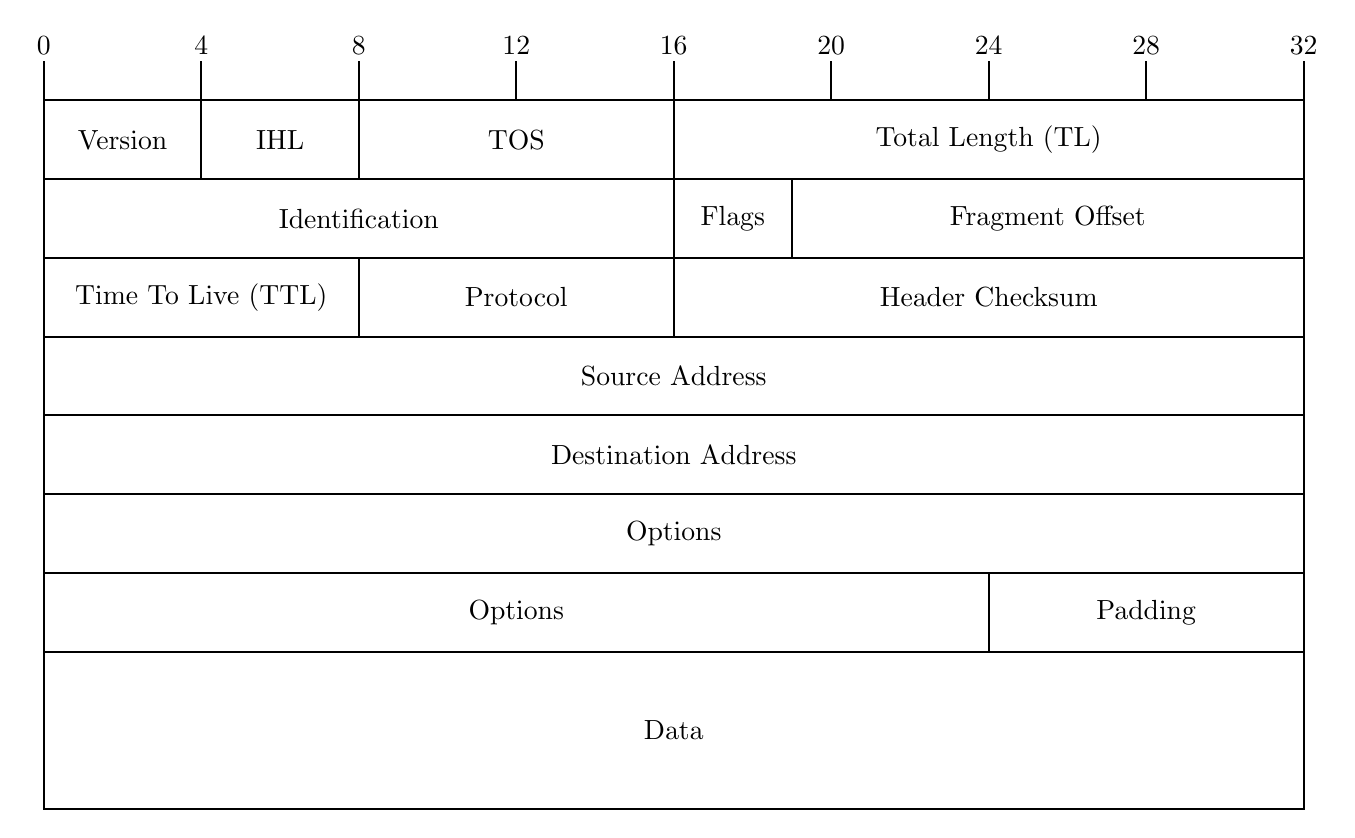
\begin{tikzpicture}
  \draw[line width = 0.75pt, align=center] (0,0) rectangle node{Data} (16,2); 
  \draw[line width = 0.75pt, align=center] (0,2) rectangle node{Options} (12,3); 
  \draw[line width = 0.75pt, align=center] (12,2) rectangle node{Padding} (16,3); 
  \draw[line width = 0.75pt, align=center] (0,3) rectangle node{Options} (16,4); 
  \draw[line width = 0.75pt, align=center] (0,4) rectangle node{Destination Address} (16,5); 
  \draw[line width = 0.75pt, align=center] (0,5) rectangle node{Source Address} (16,6);    
  \draw[line width = 0.75pt, align=center] (0,6) rectangle node{Time To Live (TTL)} (4,7); 
  \draw[line width = 0.75pt, align=center] (4,6) rectangle node{Protocol} (8,7);
  \draw[line width = 0.75pt, align=center] (8,6) rectangle node{Header Checksum} (16,7);
  \draw[line width = 0.75pt, align=center] (0,7) rectangle node{Identification} (8,8); 
  \draw[line width = 0.75pt, align=center] (8,7) rectangle node{Flags} (9.5,8); 
  \draw[line width = 0.75pt, align=center] (9.5,7) rectangle node{Fragment Offset} (16,8); 
  \draw[line width = 0.75pt, align=center] (0,8) rectangle node{Version} (2,9); 
  \draw[line width = 0.75pt, align=center] (2,8) rectangle node{IHL} (4,9);
  \draw[line width = 0.75pt, align=center] (4,8) rectangle node{TOS} (8,9); 
  \draw[line width = 0.75pt, align=center] (8,8) rectangle node{Total Length (TL)} (16,9); 
  \draw[line width = 0.75pt] (0,9.5) -- node[above=2mm]{0} (0,9);
  \draw[line width = 0.75pt] (2,9.5) -- node[above=2mm]{4} (2,9);
  \draw[line width = 0.75pt] (4,9.5) -- node[above=2mm]{8} (4,9);
  \draw[line width = 0.75pt] (6,9.5) -- node[above=2mm]{12} (6,9);
  \draw[line width = 0.75pt] (8,9.5) -- node[above=2mm]{16} (8,9);
  \draw[line width = 0.75pt] (10,9.5) -- node[above=2mm]{20} (10,9);
  \draw[line width = 0.75pt] (12,9.5) -- node[above=2mm]{24} (12,9);
  \draw[line width = 0.75pt] (14,9.5) -- node[above=2mm]{28} (14,9);
  \draw[line width = 0.75pt] (16,9.5) -- node[above=2mm]{32} (16,9);
\end{tikzpicture}
\caption{IP Segment Format}
\label{fig_SegmentFormat}
\end{figure}

\begin{description}
\item[Version: ]Gibt an, welche Version des IP Protokolls verwendet wird. (4Bit)
\item[IHL: ]Steht für Internet Header Length und gibt an, wie viele 32-Bit-Wörter von dem IP-Header belegt werden.
\item[ToS: ]Type of Service beinhaltet abstrakte Parameter zur Bestimmung der Qualität des gewünschten Services. Dabei geben die Bits Null bis Zwei die Priorität der Daten an. Die Bits Drei, Vier und Fünf stehen für niedrige Latenz, hohen Durchsatz und hohe Zuverlässigkeit. Die letztgenannten Parameter werden von Netzwerkgeräten unterschiedlich interpretiert, in den meisten Fällen ruft eine bessere Performance für einen der Parameter eine Verschlechterung bei einem anderen hervor.
\item[Paketlänge: ]Gesamtlänge eines Pakets in Bytes einschließlich des Headers. Die 16Bit ergeben eine theoretische Gesamtlänge von 65.535 Bytes, was für viele Netzwerke jedoch nicht geeignet ist. Als Mindestgröße, die alle Hosts unterstützen müssen, wurden 576 Bytes festgelegt. Das ermöglicht es, 512 Byte Daten und 64 Byte Header in einem Paket zu übertragen. Da der IP Header selber nur 20 Byte benötigt, bleibt noch ein Puffer von 44 Byte für den Header des darüber liegenden Protokolls.  
\item[Kennung: ]Ein Identifikationswert, der benötigt wird, um fragmentierte Pakete zusammen zu setzen.  (16Bit) 
\item[Flags: ]3 Bits von denen das erste reserviert ist und dauerhaft auf Null gesetzt wird. Das zweite Bit gibt an, ob das Paket fragmentiert werden darf. Das letzte Bit wird gesetzt, wenn nach dem Paket noch weitere Fragmente folgen.
\item[Fragment-Offset: ]Besteht aus 13 Bit und gibt an, an welche Stelle des Datagramms die Daten dieses Fragments gehören. 
\item[TTL ](Time-to-live): Gibt die maximale Zeit in Sekunden an, die ein Paket im Netzwerk unterwegs sein darf. Sobald die TTL den Wert Null erreicht, muss das Paket gelöscht werden. Da der Wert bei jeder Zwischenstation, unabhängig von der eigentlichen Verarbeitungszeit, ebenfalls um eins reduziert werden muss, ist die übliche Lebensdauer eines Pakets deutlich kürzer als in der TTL angegeben. 
\item[Protokoll: ]Gibt an, welches Protokoll in der darüber liegenden Ebene verwendet wird.
\item[Header Checksumme: ]Checksumme nur über den Header. Da sich der Header auf dem Weg über Zwischenstationen verändern kann, zum Beispiel wegen der Time to Live , muss die Checksumme nach jeder Verarbeitung des Headers an den Zwischenstationen neu berechnet werden.
\item[Quell-IP-Adresse: ]IP Adresse des Hosts, der das Paket ursprünglich versendet hat.(4 Byte)
\item[Ziel-IP-Adresse: ]IP Adresse des Zielendgeräts. (4 Byte)
\item[Optionen/Füllbits: ] Enthält IP-Optionen, die durch Füllbits auf 32-Bit-Wörter aufgerundet werden.
\end{description}
\cite{IPrfc}
\subsection{Adressierung}
Um mehrere Netzwerke innerhalb eines Großen zu ermöglichen, werden IP Adressen interpretiert, indem eine bestimmte Menge der höherwertigen Bits das Netzwerk spezifiziert und die restlichen Bits den genauen Host des gewählten Netzwerks adressieren. Dabei soll Flexibilität bei der Unterteilung von kleineren Teilnetzwerken ermöglicht werden. Daher wurde das Adressfeld entsprechend in bestimmte Klassen unterteilt. Es wurden drei Klassen A,B,C angelegt. Die Klassen unterscheiden sich jeweils durch die Aufteilung des Adressbereichs zwischen Netzwerk-Adresse und Host-Adresse innerhalb des Netzwerks. Die ersten 1-3 Bits der Adresse geben jeweils Aufschluss darüber, zu welcher Netzwerkklasse die jeweilige IP-Adresse gehört. Um innerhalb dieser starren Netzwerke feiner aufgeteilte Subnetze zu erzeugen, kann die Subnetmask genutzt werden. Die Subnetmask ist ebenfalls eine vier Byte große Zahl, deren niederwertige Bits auf Null gesetzt werden und damit den variablen Teil innerhalb des Subnets angeben. Der Rest der Maske wird dabei auf Eins gesetzt.\cite{IPrfc}

\subsection{Fragmentierung}

Paketfragmentierung wird nötig, wenn ein Paket aus einem Netzwerk kommt, das eine große maximale Segmentgröße erlaubt und durch eines geleitet wird, das nur eine kleinere Segmentgröße erlaubt. Dabei können die Pakete in eine theoretisch nahezu endlose Anzahl von kleinen Paketen zerlegt werden, wobei die Datenblöcke aller Fragmente abgesehen vom letzten ein Vielfaches von 64 Byte an Daten beinhalten müssen.\\\\
\begin{figure}[htp]
	\centering
	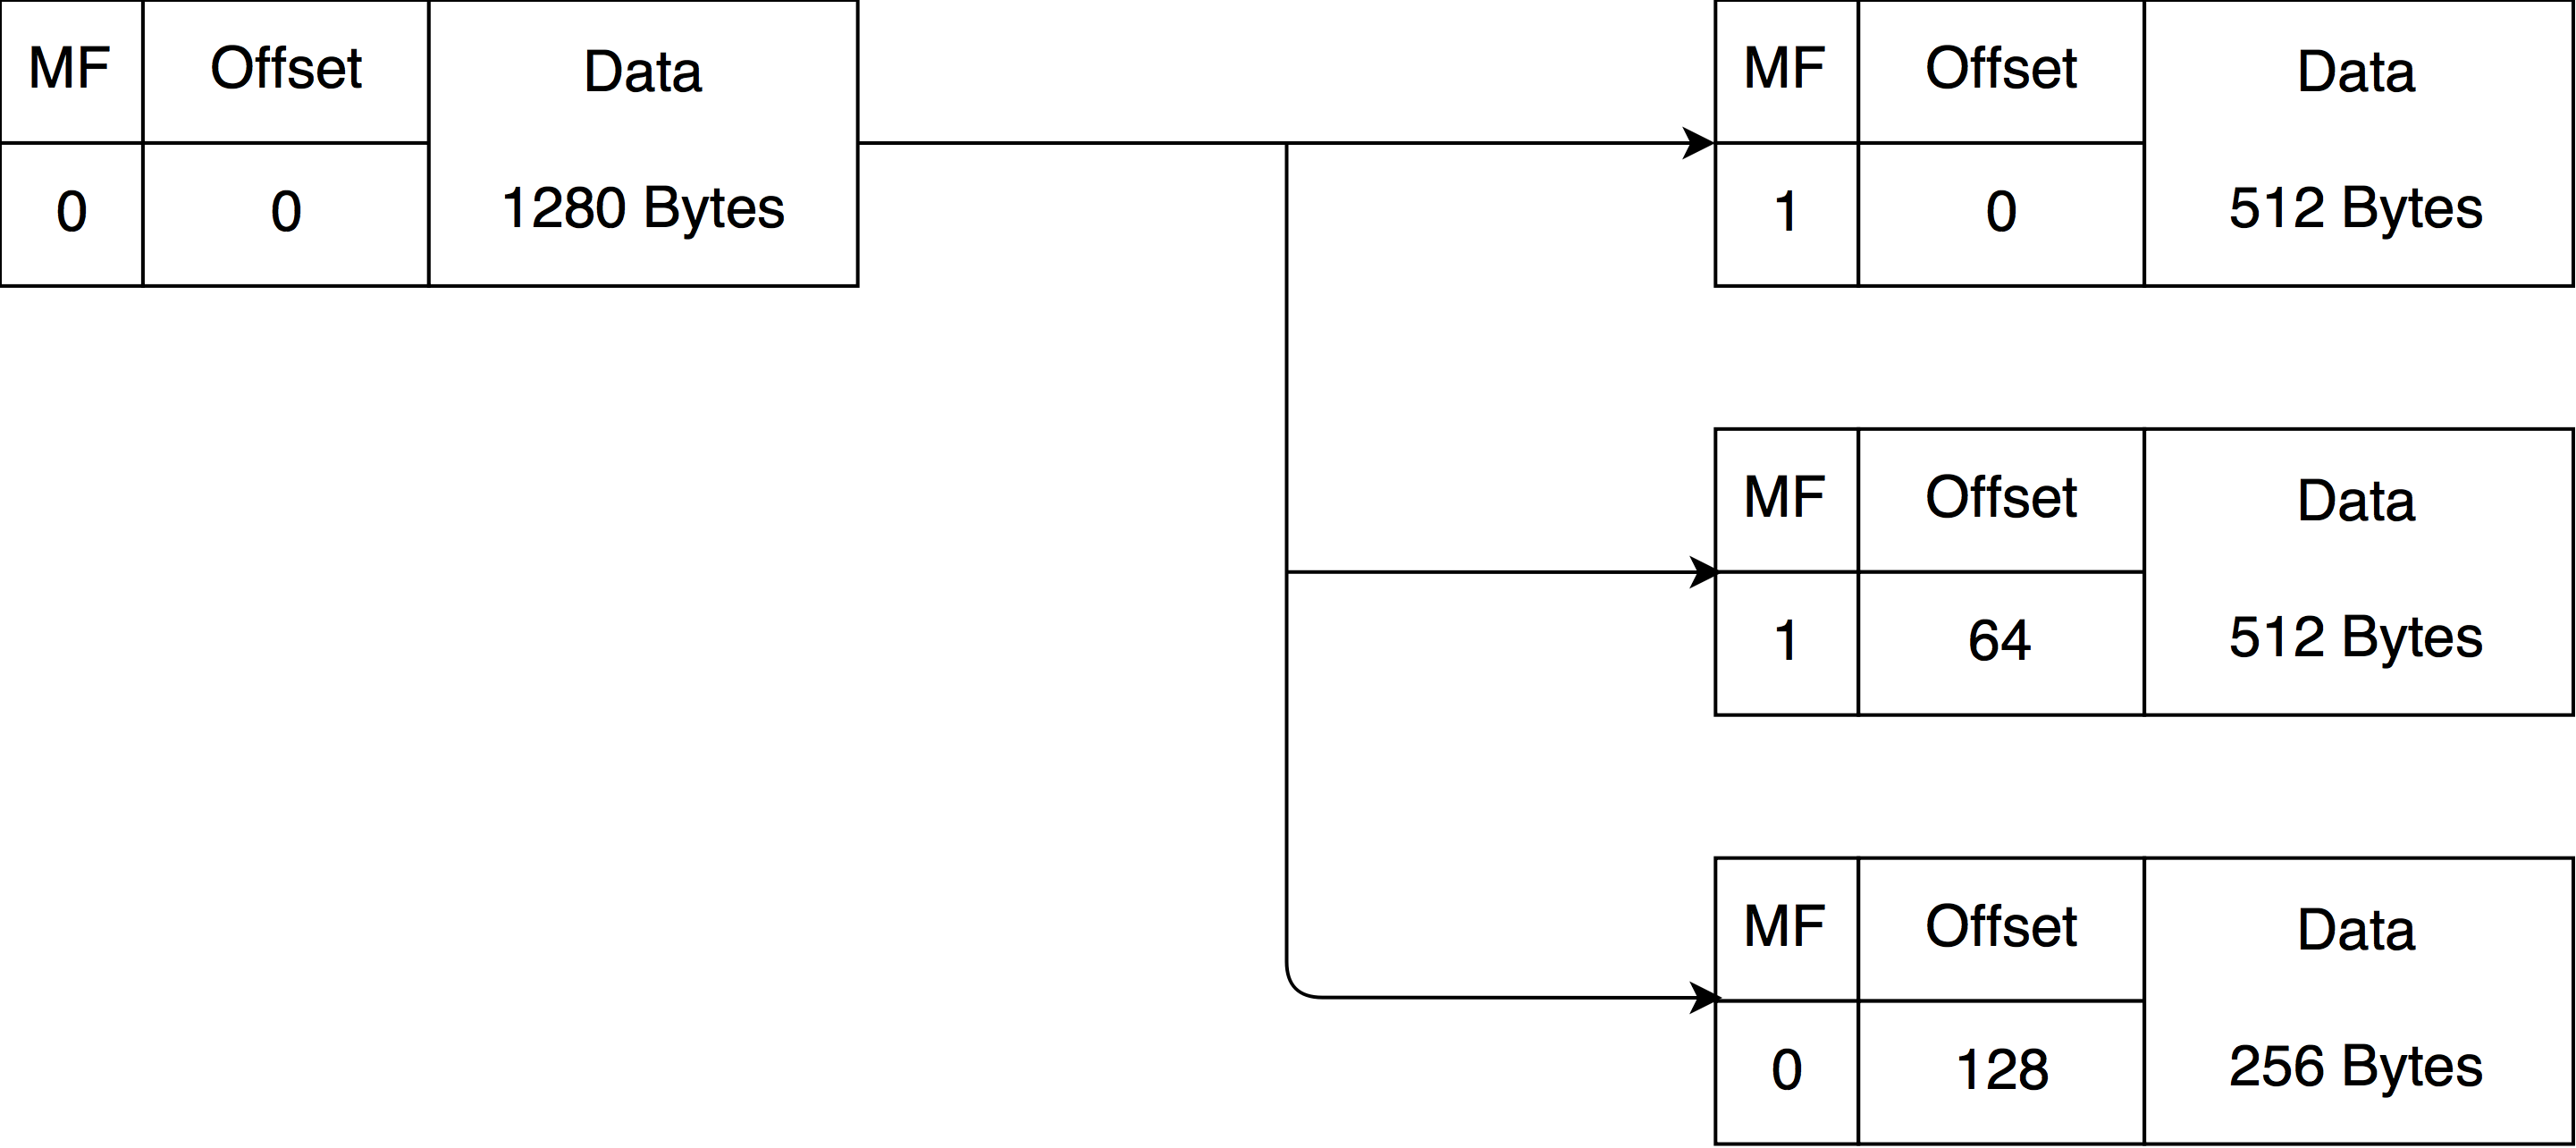
\includegraphics[width=0.75\textwidth]{Graphics/IPfragmentation.png}
	\caption{IP-Paket Fragmentierung}
\end{figure}
Damit fragmentierte Paket richtig zusammengesetzt werden können, haben alle Fragmente eines Pakets die gleiche Identifikationsnummer. Für das Zusammensetzen des Datenblock wird der Fragmentoffset benötigt, der angibt, an welcher Stelle des ursprünglichen Datenblocks die Daten des Fragments stehen. Das fragmented-flag sagt dabei aus, ob noch weitere Fragmente folgen, oder ob dies das letzte Teil ist. Sobald alle Fragmente eines Pakets beim Ziel eingetroffen sind, kann das ursprüngliche Paket wiederhergestellt werden.\cite{IPrfc} 

\FloatBarrier
\section{Transmission Control Protocol (TCP)}
Da die Protokolle der unteren Schichten, IP und Ethernet, keine fehlerfreie und verlustlose Übertragung der Daten garantieren können, wird ein Protokoll auf der Transportschicht benötigt, das eine zuverlässige Übertragung von Daten zwischen Anwendungen auf entfernten Hosts sicherstellen kann, auch wenn auf jedem Host eine große Anzahl an Anwendungen läuft, die TCP verwenden. Für diesen Zweck wurde das TCP-Protokoll erschaffen. Um dabei die Datenpakete jeweils der richtigen Anwendung zuordnen zu können werden Port-Nummern verwendet.\cite{TCPr} \\\\
Es handelt sich bei TCP um ein verbindungsorientiertes Protokoll. Das bedeutet, dass es zu Beginn einer Übertragung einen klar definierten Verbindungsaufbau gibt. Nachdem die Verbindung etabliert ist, können Daten vollduplex übertragen werden. Wobei durch Sequenz-Nummern und Acknowledge-Nummern die richtige Reihenfolge und Vollständigkeit der Datenpakete sichergestellt wird. Pakete, deren Erhalt nicht bestätigt wurde, werden automatisch neu übertragen. Des weiteren verfügt TCP über Mechanismen, um eine Überlast auf dem Übertragungsweg rechtzeitig zu erkennen und zu beheben.\cite{TCPr}   

\subsection{Paketaufbau}


\begin{description}

\item[Quell Port (16Bit): ] Gibt die Portnummer der Anwendung auf Senderseite an. 
\item[Ziel Port (16Bit): ] Gibt die Portnummer der Anwendung auf Empfängerseite an.
\item[Sequence Number (32Bit): ] Gibt die Sequenz-Nummer des Pakets an.
\item[Acknowledge Number (32Bit): ] Gibt die Acknowledge Nummer des Pakets an.
\item[Data Offset (4Bit): ] Anzahl von 32Bit Wörtern aus denen der Header besteht. 
\item[Reserved (6Bit): ] reserviert für zukünftige Nutzung
\item[Steuerungsbits (6Bit): ] Sechs Flags die für die Ablauf-Steuerung der Übertragung genutzt werden: 
\begin{figure}[htp]
\centering
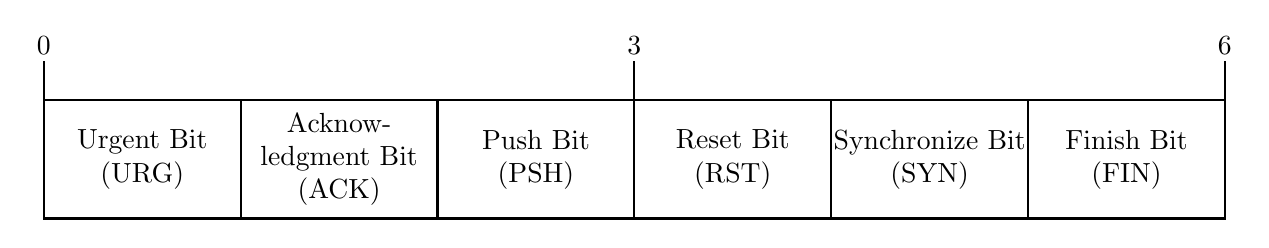
\begin{tikzpicture}
  \draw[line width = 0.75pt, align=center] (0,0) rectangle node{Urgent Bit\\(URG)} (2.5,1.5); 
  \draw[line width = 0.75pt, align=center] (2.5,0) rectangle node{Acknow-\\ ledgment Bit\\(ACK)} (5,1.5);
  \draw[line width = 0.75pt, align=center] (5,0) rectangle node{Push Bit\\(PSH)} (7.5,1.5);
  \draw[line width = 0.75pt, align=center] (7.5,0) rectangle node{Reset Bit\\(RST)} (10,1.5);
  \draw[line width = 0.75pt, align=center] (10,0) rectangle node{Synchronize Bit\\(SYN)} (12.5,1.5);
  \draw[line width = 0.75pt, align=center] (12.5,0) rectangle node{Finish Bit\\(FIN)} (15,1.5);
  \draw[line width = 0.75pt] (0,2) -- node[above=2mm]{0} (0,1.5);
  \draw[line width = 0.75pt] (7.5,2) -- node[above=2mm]{3} (7.5,1.5);
  \draw[line width = 0.75pt] (15,2) -- node[above=2mm]{6} (15,1.5);
\end{tikzpicture}
\caption{TCP Control Bits}
\label{fig_ControlBits}
\end{figure}
\begin{itemize}
\item[URG: ] Urgent Pointer, wird in moderner Software nicht mehr genutzt und wird von vielen Implementierungen ignoriert. 
\item[ACK: ] Acknowledgment gibt an, ob das Paket eine gültige Bestätigung für empfangene Pakete enthält.
\item[PSH: ] Ist dieses Flag gesetzt, werden die empfangenen Daten sofort an die Hostsoftware weitergereicht. 
\item[RST: ] Wird im Fehlerfall gesendet und bricht die Verbindung ab. 
\item[FIN: ] Signalisiert das Ende der Verbindung, wenn es keine zu übertragenen Daten gibt. 
\end{itemize}
\item[Window (16Bits): ] Gibt die Größe des Empfangs-Windows des Absenders an. Gilt für den Empfänger als obere Grenze des Congestion-Windows.
\item[Checksum (16Bits): ] Für die Berechnung der Checksumme über das TCP Paket wird vorher ein Pseudoheader bestehend aus der Quell- und Ziel IP-Adresse, des IP-Codes für das verwendete Protokoll und die Gesamtlänge des eigentlichen TCP-Pakets berechnet. Die Checksumme wird daraufhin über den Pseudoheader, den Header und die Payload berechnet. Dafür werden diese in 16 Bit große Blöcke aufgeteilt und im Einer-Komplement die Summe über diese gebildet. 
\item[UrgentPointer (16Bits): ] Gibt den Urgentpointer als Offset zu der Sequenznummer an. Wird nur interpretiert, wenn das URG Flag gesetzt ist.\
\item[Options: (Variabel): ]  Optionale Informationen, die von TCP Implementierungen unterstützt werden können, um Sicherheit und Performance zu verbessern. Optionen bestehen entweder nur aus einem Optionsbyte oder haben zusätzlich ein weiteres Byte, das die Länge der jeweiligen Option angibt. 
\item[Padding: ] Falls der TCP Header mit den Optionen einen teilweise genutzten 32Bit Block hat, wird dieser mit Nullen aufgefüllt. \cite{TCPr} 
\end{description}
\begin{figure}[htp]
\centering
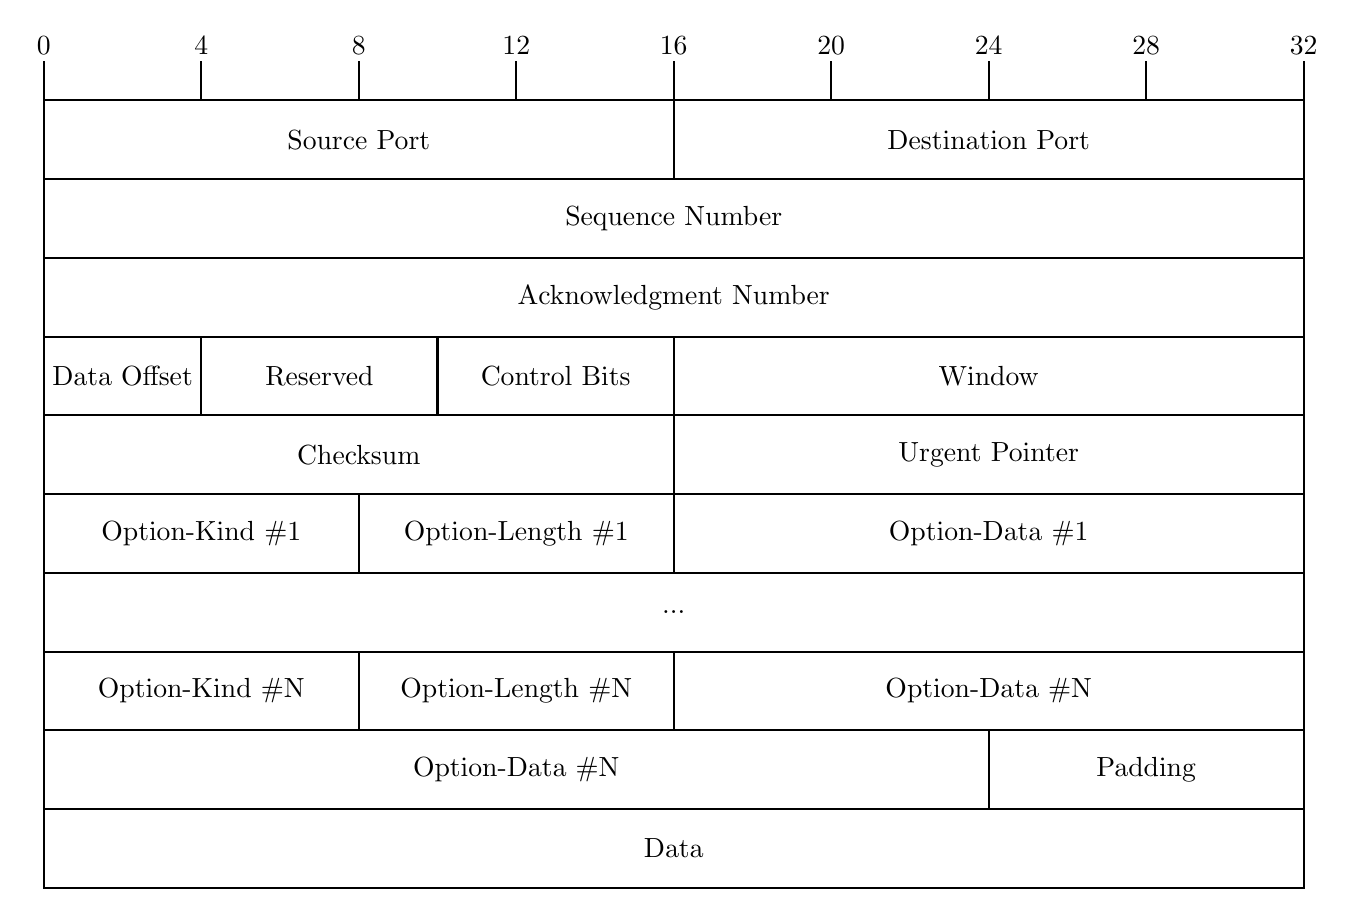
\begin{tikzpicture}
  \draw[line width = 0.75pt, align=center] (0,0) rectangle node{Data} (16,1); 
  \draw[line width = 0.75pt, align=center] (0,1) rectangle node{Option-Data \#N} (12,2); 
  \draw[line width = 0.75pt, align=center] (12,1) rectangle node{Padding} (16,2); 
  \draw[line width = 0.75pt, align=center] (0,2) rectangle node{Option-Kind \#N} (4,3); 
  \draw[line width = 0.75pt, align=center] (4,2) rectangle node{Option-Length \#N} (8,3); 
  \draw[line width = 0.75pt, align=center] (8,2) rectangle node{Option-Data \#N} (16,3); 
  \draw[line width = 0.75pt, align=center] (0,3) rectangle node{...} (16,4); 
  \draw[line width = 0.75pt, align=center] (0,4) rectangle node{Option-Kind \#1} (4,5); 
  \draw[line width = 0.75pt, align=center] (4,4) rectangle node{Option-Length \#1} (8,5); 
  \draw[line width = 0.75pt, align=center] (8,4) rectangle node{Option-Data \#1} (16,5);   
  \draw[line width = 0.75pt, align=center] (0,5) rectangle node{Checksum} (8,6); 
  \draw[line width = 0.75pt, align=center] (8,5) rectangle node{Urgent Pointer} (16,6);
  \draw[line width = 0.75pt, align=center] (0,6) rectangle node{Data Offset} (2,7); 
  \draw[line width = 0.75pt, align=center] (2,6) rectangle node{Reserved} (5,7); 
  \draw[line width = 0.75pt, align=center] (5,6) rectangle node{Control Bits} (8,7); 
  \draw[line width = 0.75pt, align=center] (8,6) rectangle node{Window} (16,7);
  \draw[line width = 0.75pt, align=center] (0,7) rectangle node{Acknowledgment Number} (16,8); 
  \draw[line width = 0.75pt, align=center] (0,8) rectangle node{Sequence Number} (16,9); 
  \draw[line width = 0.75pt, align=center] (0,9) rectangle node{Source Port} (8,10); 
  \draw[line width = 0.75pt, align=center] (8,9) rectangle node{Destination Port} (16,10); 
  \draw[line width = 0.75pt] (0,10.5) -- node[above=2mm]{0} (0,10);
  \draw[line width = 0.75pt] (2,10.5) -- node[above=2mm]{4} (2,10);
  \draw[line width = 0.75pt] (4,10.5) -- node[above=2mm]{8} (4,10);
  \draw[line width = 0.75pt] (6,10.5) -- node[above=2mm]{12} (6,10);
  \draw[line width = 0.75pt] (8,10.5) -- node[above=2mm]{16} (8,10);
  \draw[line width = 0.75pt] (10,10.5) -- node[above=2mm]{20} (10,10);
  \draw[line width = 0.75pt] (12,10.5) -- node[above=2mm]{24} (12,10);
  \draw[line width = 0.75pt] (14,10.5) -- node[above=2mm]{28} (14,10);
  \draw[line width = 0.75pt] (16,10.5) -- node[above=2mm]{32} (16,10);
\end{tikzpicture}
\caption{TCP Segment Format}
\label{fig_SegmentFormat}
\end{figure}

\FloatBarrier
\subsection{Zustände}
TCP ist im Gegensatz zu den bisher genannt Protokollen zustandsorientiert, was bedeutet, dass es je nach Zustand anders auf Nutzeraktionen und ankommende Pakete reagiert. 
Zu den Zuständen gehören :\cite{TCPr,TCPm} 



\begin{description}

\item[CLOSED: ]Das ist der Startzustand einer TCP Instanz. Die Verbindung ist geschlossen. Usercalls außer \textit{Open} werden mit Fehlermeldungen quittiert und ankommende Pakete werden verworfen und mit einem Reset-Paket beantwortet.
\item[SYN-SENT: ]Nachdem eine Verbindung initiiert wurde, wird auf eine Antwort des {}"remote Hosts"{} gewartet. 
\item[SYN-RECEIVED: ] Nachdem ein SYN Paket erhalten und ein SYN-ACK gesendet wurde, wird auf das ACK gewartet, um den 3-Wege-Handschlag abzuschließen. 
\item[ESTABLISHED: ] Nach dem der Verbindungsaufbau erfolgreich abgeschlossen wurde, befinden sich beide Hosts im ESTABLISHED Zustand, in dem eine Vollduplex Kommunikation möglich ist. 
\item[FIN-WAIT-1: ] Wenn ein Verbindungsabbau initiiert wurde, wird ein FIN Paket gesendet, in den Zustand FIN-WAIT-1 gewechselt und auf die Bestätigung des Erhalts gewartet. 
\item[FIN-WAIT-2: ] Falls die Gegenstelle noch Daten zu übertragen hat, bleibt die Verbindung einseitig offen, um die letzten Pakete zu empfangen. 
\item[CLOSING: ]	Wartet auf das letzte ACK-Paket und wechselt, wenn dieses ankommt in den Zustand TIME-WAIT.
\item[TIME-WAIT: ] Hält die Verbindung nach Beendigung einige Minuten offen, um auf verzögerte Pakete zu reagieren.
\end{description}\cite{TCPr,TCPm} 

\subsection{Nutzeraufrufe}
Zu den Zuständen kommen noch eine Reihe von Ereignissen, auf die, abhängig von den jeweiligen Zuständen, entsprechend reagiert werden muss. 
Dazu gehören neben eintreffenden Paketen und Timeouts die Usercalls.
\begin{description}
\item[Active OPEN: ]Öffnet einen Port und initiiert den Verbindungsaufbau zu einem Remote Host.
\item[Passive OPEN: ] Öffnet einen Port ohne eine Verbindung zu initiieren und wartet auf einen Verbindungsaufbau,
\item[SEND: ] Fügt dem Sendepuffer Daten hinzu und sendet gegebenenfalls ein Datenpaket.
\item[RECEIVE: ] Überprüft, ob genug Daten vorhanden sind und gibt diese an die Anwendung zurück.
\item[CLOSE: ] Initiiert den Abbau der Verbindung, wenn es keine Daten mehr zu  übertragen gibt.
\item[ABORT: ] Bricht die Verbindung ab. In den meisten Zuständen wird in dem Fall ein Reset Paket gesendet.
\end{description}\cite{TCPr,TCPm} 

\begin{figure}[htp]
	\centering
	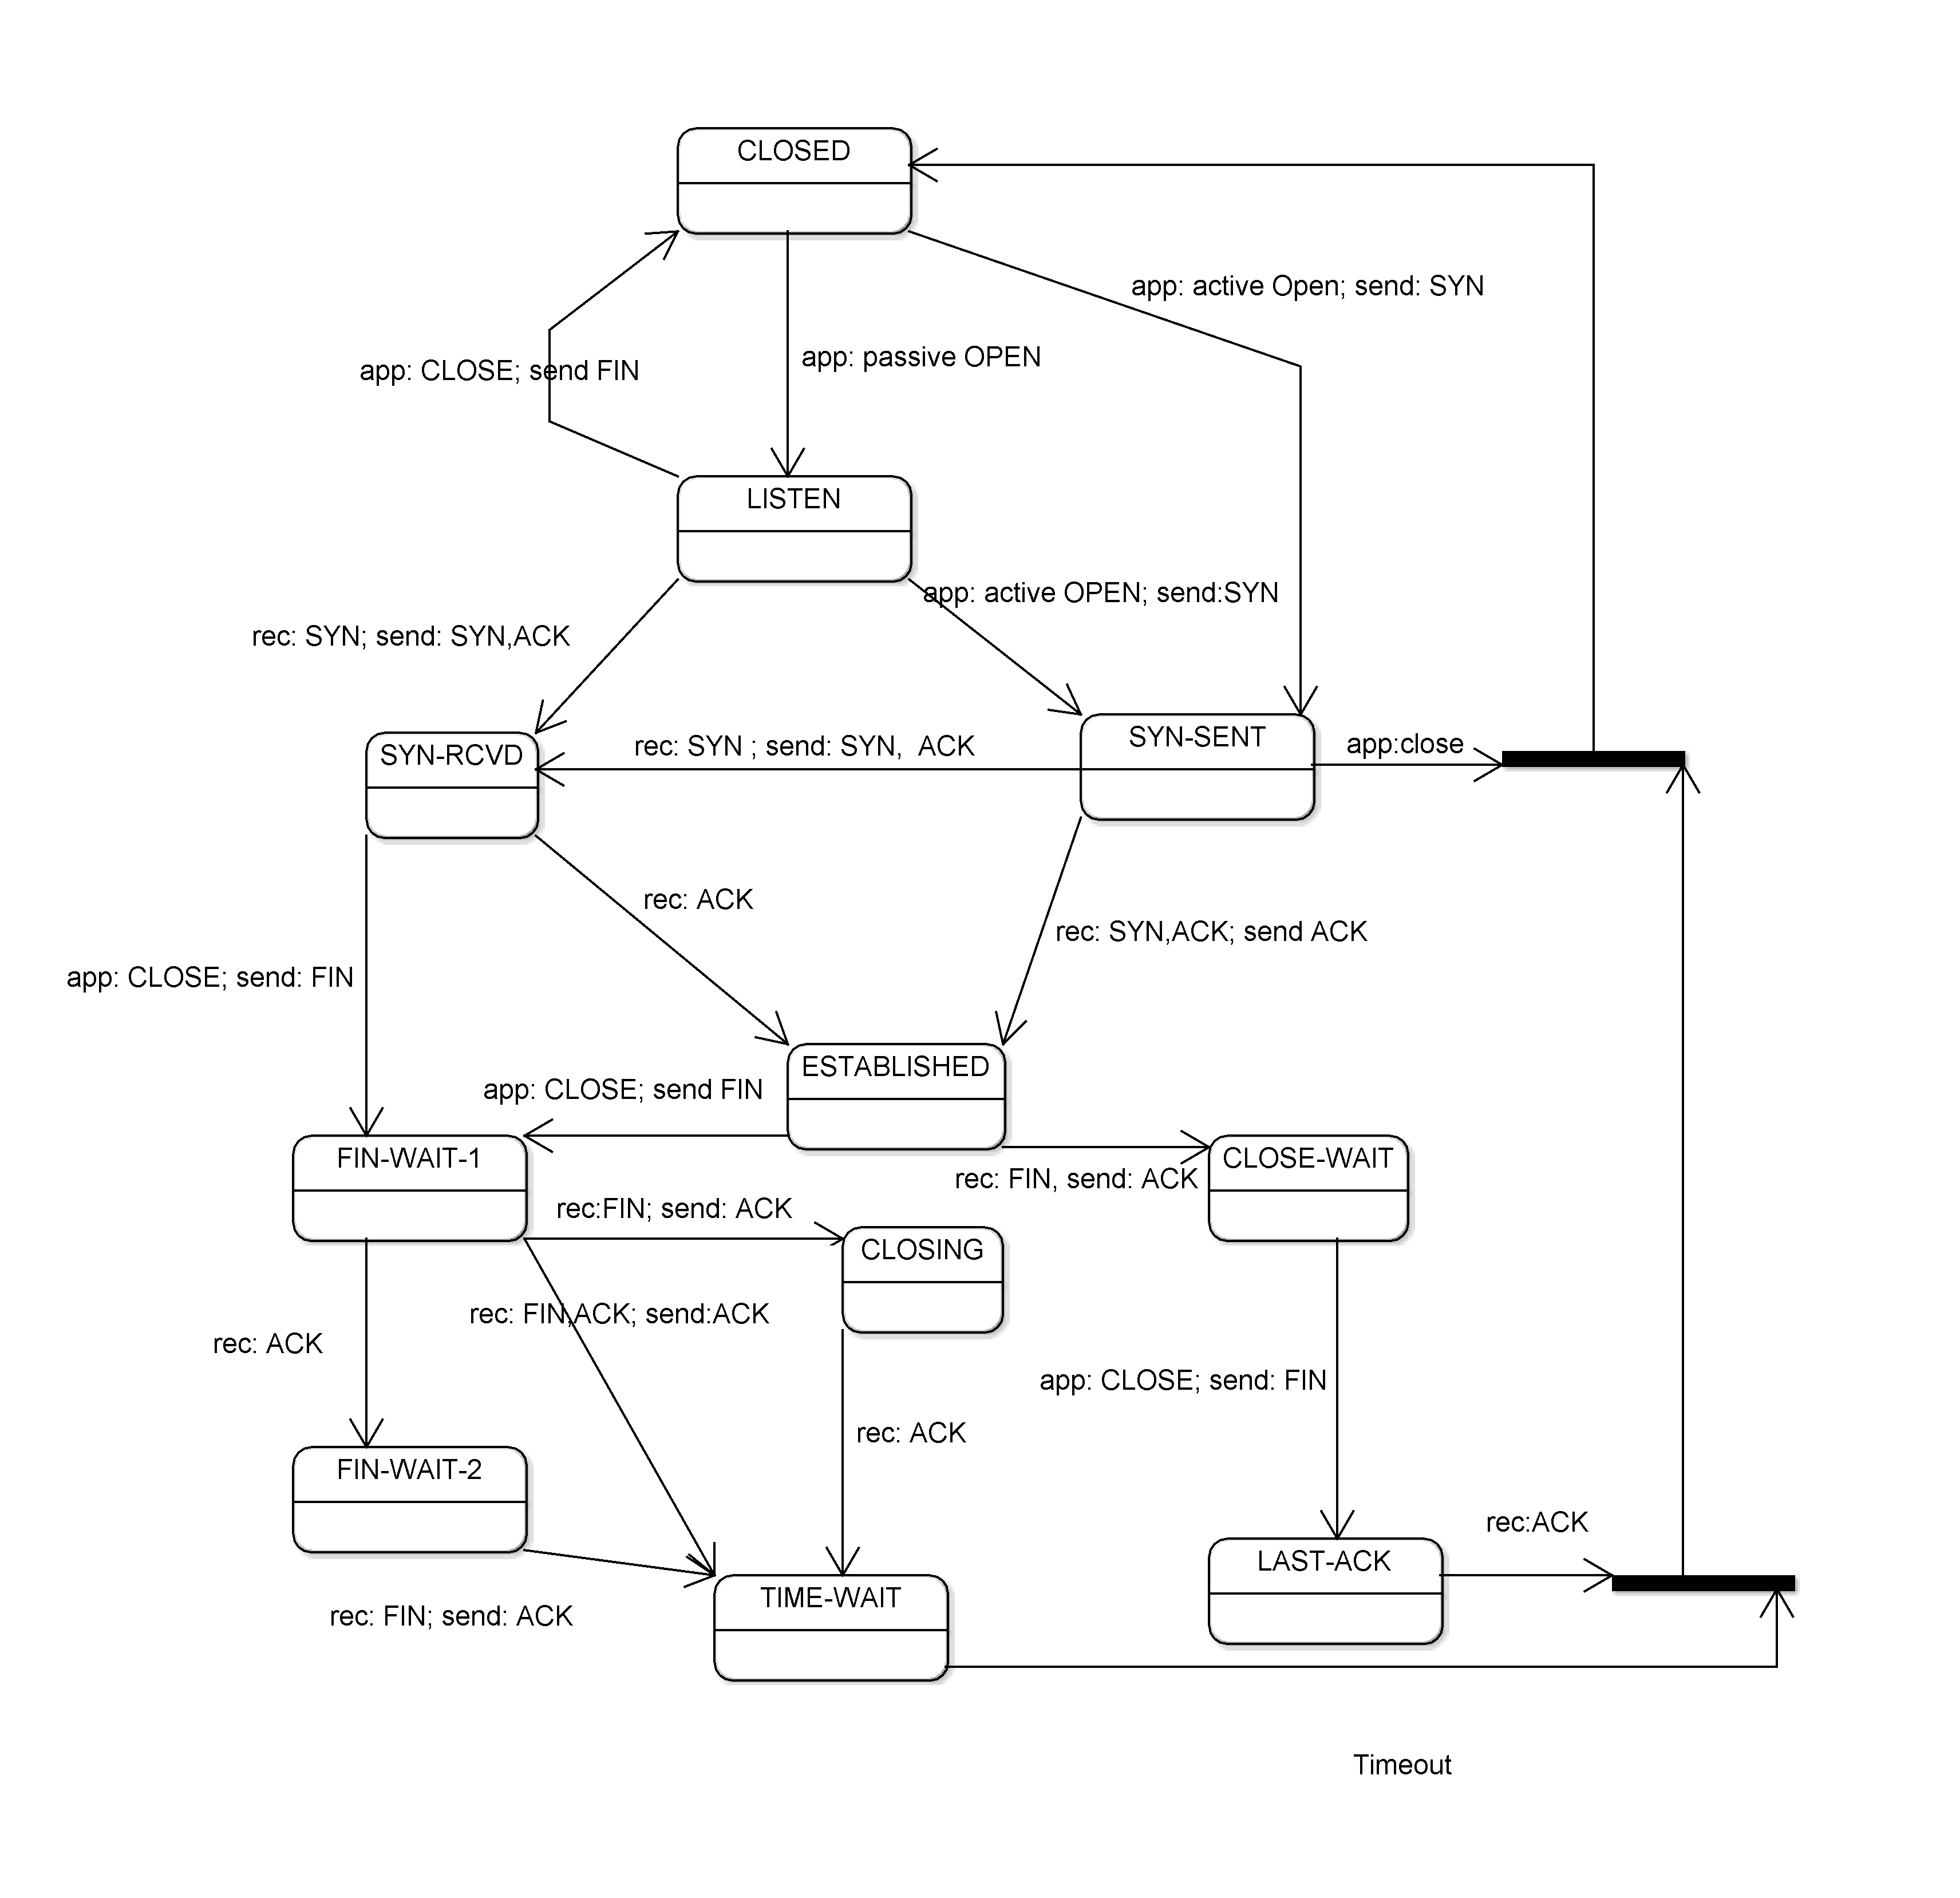
\includegraphics[width=1\textwidth]{Graphics/tcp_Statemachine.png}
	\caption{vereinfachter Zustandsautomat TCP}

\end{figure}
\FloatBarrier
\subsection{Sequenznummern}
Ein wichtiges Grundprinzip von TCP ist, dass jedem Byte an Daten eine eigene Sequenznummer zugewiesen werden kann. Dadurch ist es möglich, dass jedes Byte einzeln bestätigt werden kann. Der in TCP dazu verwendete Mechanismus arbeitet kumulativ. Das bedeutet, wenn eine Sequenznummer bestätigt wird, gelten alle Sequenznummern kleiner als die Bestätigungsnummer als angekommen. Dadurch wird es einfach, den Verlust einzelner Pakete zu erkennen und diese nochmal zu senden. Das erste Byte eines Datenpaketes entspricht dabei der Sequenznummer des Pakets. \cite{TCPr} 

\subsection{Verbindungsaufbau}
Um zuverlässig einen sicheren Verbindungsaufbau zu gewährleisten, verwendet TCP einen Drei-Wege-Handshake. Soll eine neue Verbindung aufgebaut werden, wird die Initiale Sequenznummer zuverlässig generiert. Das SYN-Paket enthält nur den HEADER mit der um eins inkrementierten, initialen Sequenznummer und den SYN-Flag. Nach dem Sendevorgang wird in den Zustand SYN-SENT gewechselt. Wenn die Empfängerseite sich im Zustand LISTEN befindet, kann die Verbindungsanfrage bestätigt werden. Dafür wird ebenfalls eine initiale Sequenznummer generiert. Zur Antwort wird ein Paket erzeugt, das die neue initiale Sequenznummer verwendet und als Acknummer die um eins erhöhte Sequenznummer des SYN-Pakets verwendet. Die Flags für SYN und ACK werden gesetzt. Nach dem Senden wird in den Zustand SYN-RECEIVED gewechselt.\\
Nach dem Erhalt des SYN-ACK-Pakets sendet die initiierende Seite ein leeres ACK-Paket und wechselt in den ESTABLISHED Zustand. \cite{TCPr} 

\begin{figure}[h]
	\centering
	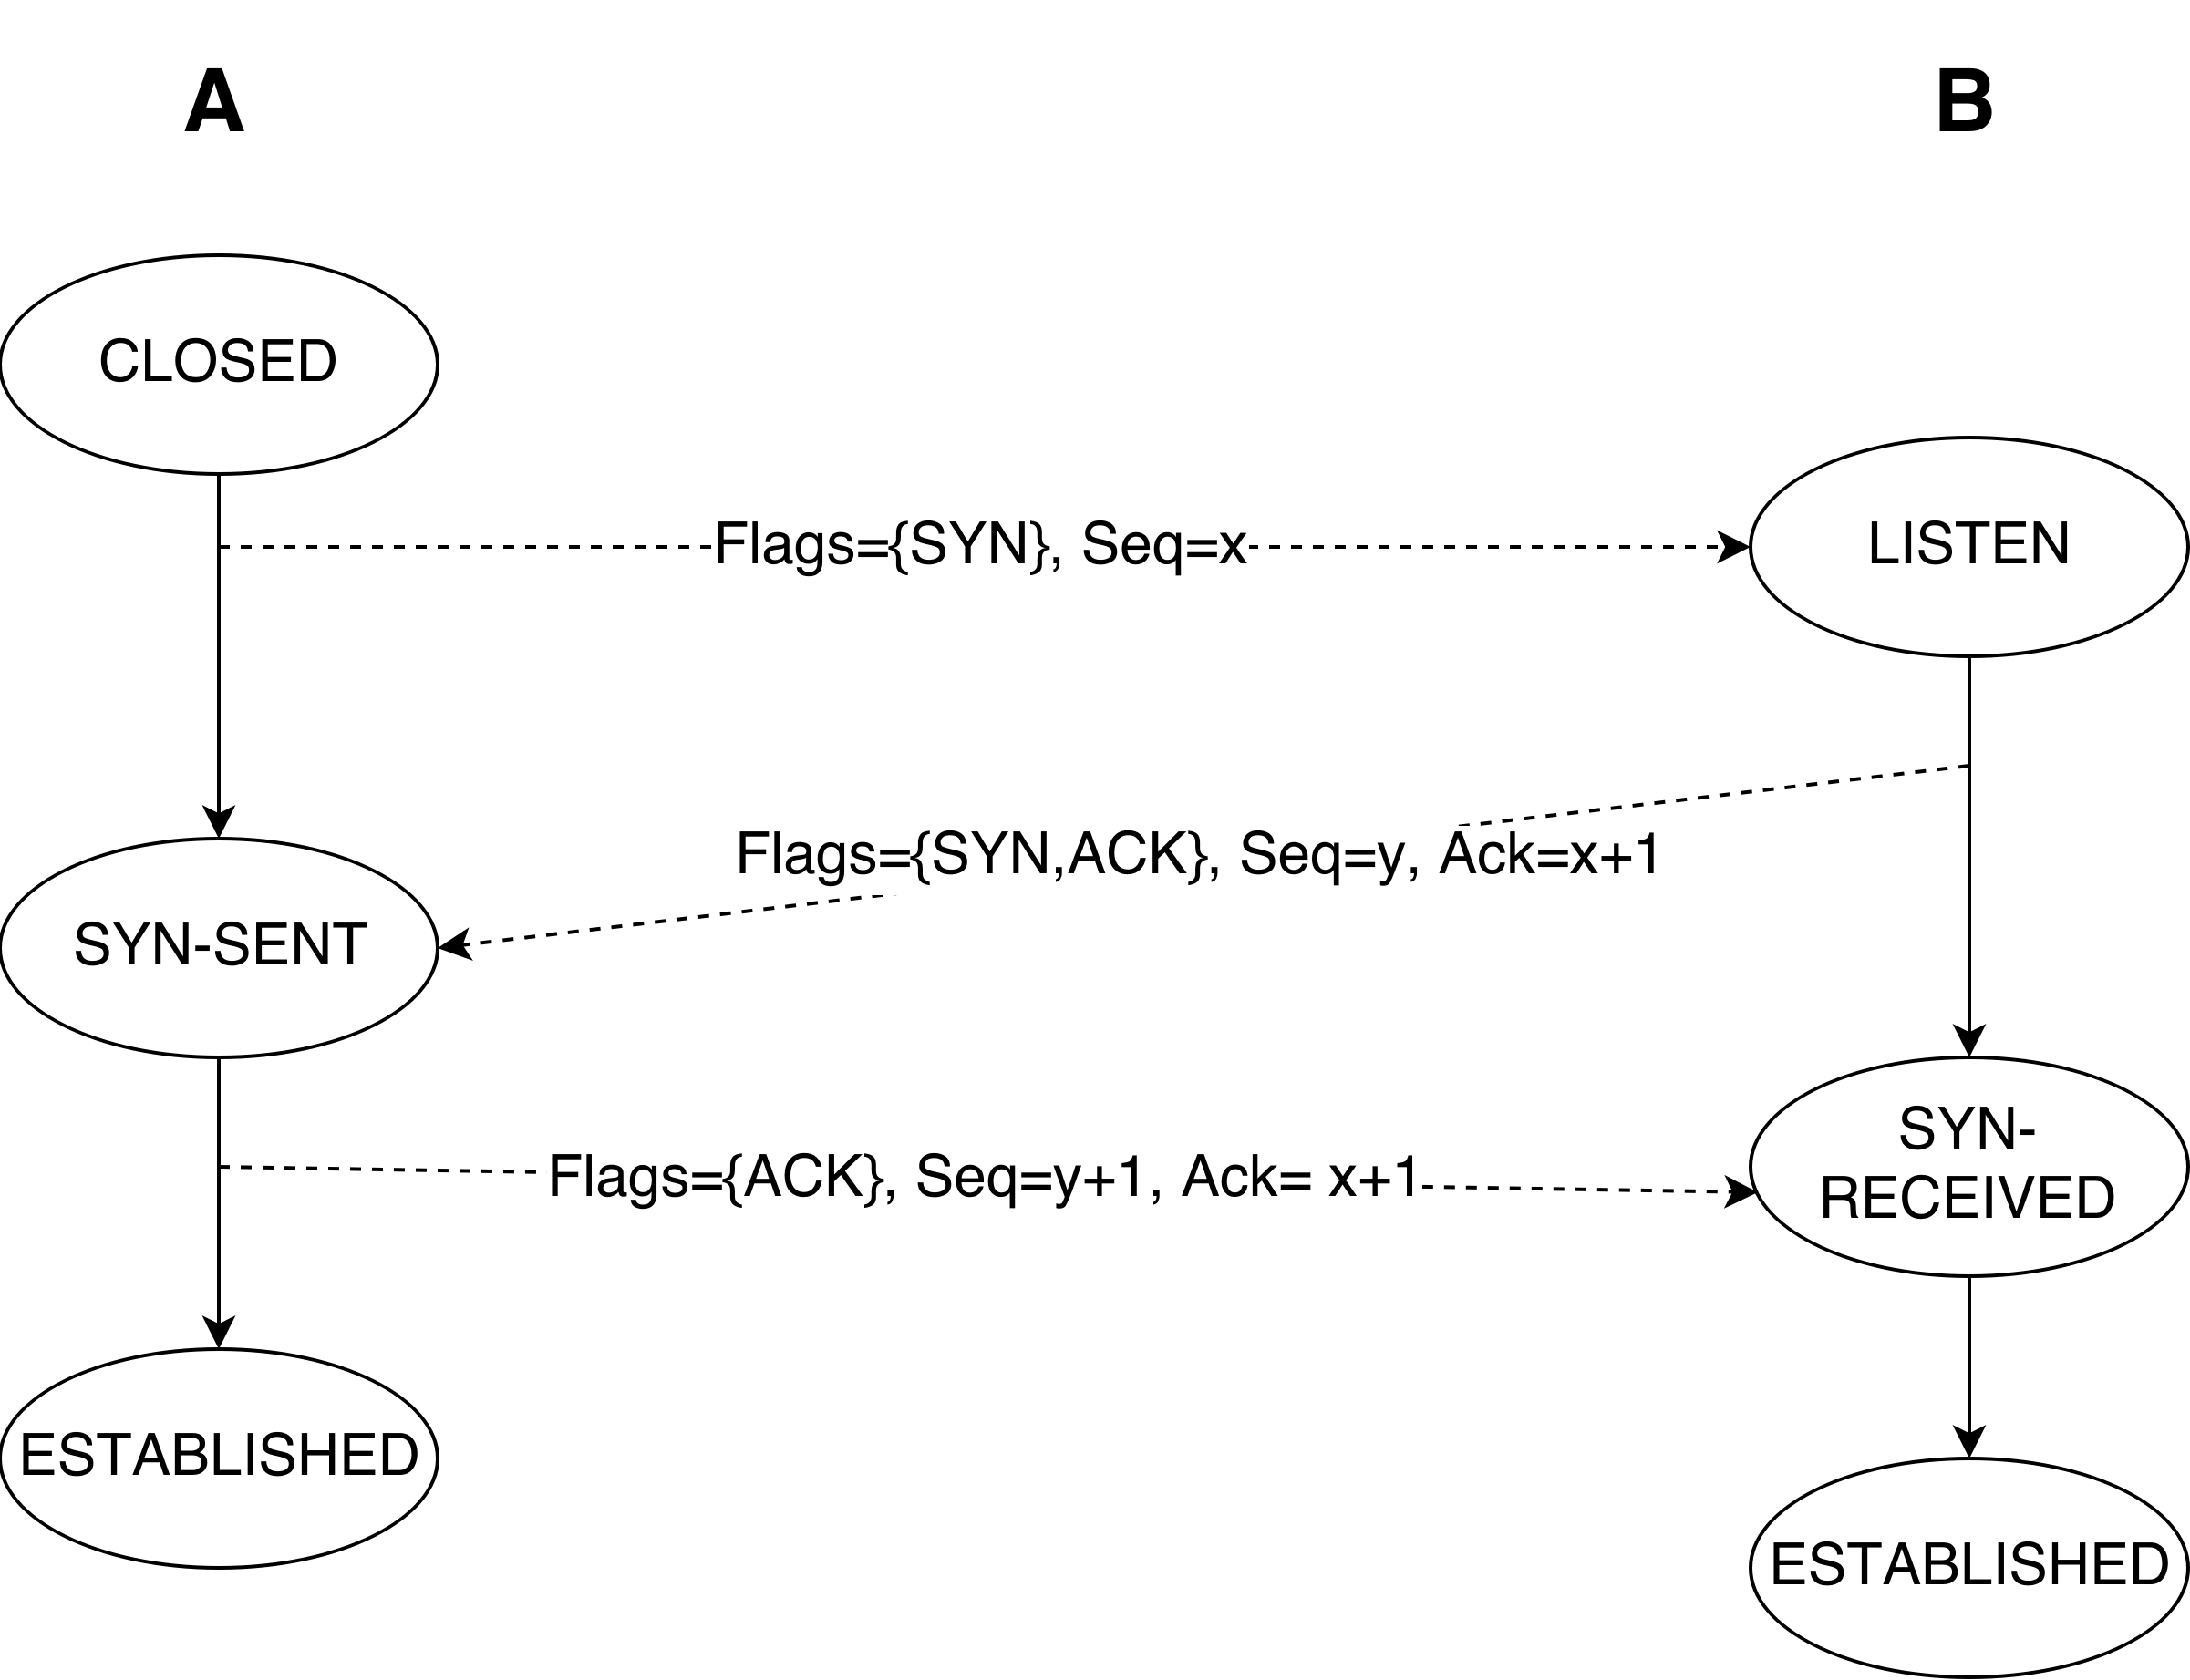
\includegraphics[width=0.6\textwidth]{Graphics/tcp_Handshake.png}
	\caption{TCP Handshake mit Zustandstransitionen}
\end{figure}
\FloatBarrier
\subsection{Datenübertragung}

Wenn beide Seiten einer Verbindung den Established-Zustand erreicht haben, kann die eigentliche beidseitige Datenübertragung beginnen. Dabei wird die Übertragung der Daten als kontinuierlicher Datenstrom abstrahiert. Eine Anwendung schreibt dabei Bytes auf einen Datenpuffer im TCP-Stack. Die Daten werden nicht sofort übertragen, da sonst viele Pakete mit wenig Nutzdaten gesendet würden und die Verbindung schnell überlastet wäre, wobei ein großer Teil der übertragenen Daten für den durch TCP-, IP- und Ethernet-Header erzeugten Overhead genutzt werden müssten. Sobald der Schreibpuffer eine bestimmte Größe erreicht hat oder die Software einen PUSH signalisiert, wird ein TCP-Paket erzeugt, das die Daten aus dem Puffer überträgt. Jedes Datenpaket wird mit einem Zeitstempel in der Retransmitqueue zwischengespeichert, bis der Erhalt des Pakets bestätigt wurde. Nach dem Eintreffen eines Pakets, dessen ACK-Flag gesetzt wurde, gelten alle Pakete, deren Sequenznummer unter der Acknowledge-Nummer des angekommenen Paktes liegen, als bestätigt. Diese werden aus der Retransmitqueue entfernt. Wenn für ein Paket eine bestimmte Zeit lang keine Bestätigung eingetroffen ist, wird dieses nochmal gesendet.\cite{TCPr}  

\subsection{Überlastkontrolle}

Ein weiterer Schwerpunkt bei TCP ist das Verhindern der Überlastung des Netzwerks, das zwischen Sender und Empfänger liegt, als auch die des Empfängers selber. 
Die beiden Mechanismen werden "{}Flow Control"{} und "{}Congestion Control"{} genannt. 
{}"Flow Control{}" verhindert dabei die Überlastung des Empfängers und "{}Congestion Control"{} die des Übertragungsweges. \\\\
Für das Senden von Daten wird für "{}Flow"{} und "{}Congestion Control"{} jeweils ein Fenster bestimmt. Das Fenster gibt an, wie viele Bytes gesendet werden können, ohne dass die vorherigen bestätigt wurden. Wenn die Differenz der Sequenznummern und der letzten erhaltenen Acknowledgenummer so groß ist wie das Fenster, werden keine neuen Datenpakete mehr versendet, bis weitere Pakete bestätigt wurden. Es wird jeweils das kleinere Fenster als Grenze genommen. \\\\
Die Größe des Flow {}"Control Windows"{} des Empfänger wird im TCP Header der von ihm versendeten Pakete angegeben. 
Das Problem bei der "{}Congestion Control"{} ist, dass die Kapazität der Verbindung nicht trivial zu bestimmen ist. Für eine Annäherung kommen im Normalfall vier Algorithmen zum Einsatz. Mit Hilfe der Variable \textit{Slow Start Threshold} wird festgelegt, welcher der Algorithmen zu diesen Zeitpunkt zum Einsatz kommt. So lange die Größe des \textit{Congestion Windows} unter der \textit{Slow-Start-Threshold} liegt, wird der "{}Slow Start"{} Algorithmus verwendet. Eine Überlastung der Verbindung kann festgestellt werden, wenn mehrere Acknowledge Pakete für dieselbe Sequenznummer empfangen werden.\\\\
Zu Beginn einer Übertragung liegen noch keine Informationen über die mögliche Bandbreite des Netzwerks vor, weswegen die Bandbreite langsam sondiert werden muss. Dabei wird der "{}Slow Start"{}-Algorithmus genutzt, bis durch schnelles Ansteigen der Übertragungsrate der Grenzwert erreicht wird. Die "{}Slow Start"{}-Phase wird genutzt, bis die Größe des \textit{Congestion Windows} die \textit{Slow-Start-Threshold} übersteigt oder eine Überlastung der Verbindung festgestellt wird. Da die Grenze der Verbindungskapazität sondiert werden soll, wird die \textit{Slow-Start-Threshold} zu Beginn auf einen Wert gesetzt, der nicht erreicht werden kann. Wenn es zu einen Packet Timeout kommt, wird die \textit{Slow Start Threshold} auf einen Wert, der einem Bruchteil des erreichten Fensters entspricht, gesetzt und der "{}Slow Start"{} Algorithmus mit einem größeren initialen Fenster weiter verwendet. Diesmal wird die "{}Slow Start Phase"{} durch das Überschreiten der \textit{Slow-Start-Threshhold} beendet. Für den Rest der Übertragung wechseln sich die beiden Algorithmen ab, bis die Verbindung beendet ist.\\\\
Es gibt eine Reihe von Varianten für die Congestion Control Implementierung. Alle davon verwenden eine Variation der folgenden Algorithmen. Hier wird als Beispiel die Reno Variante genannt.\cite{TCPr,cc} 

\begin{description}
\item[Slow Start: ] Vergrößert das \textit{Congestion Window} mit jedem bestätigten Segment um die Größe des Segments. Effektiv eine Verdoppelung des Windows pro Roundtrip.
N := Anzahl der im letzten Ack bestätigten Sequenznummern
\item[Congestion Avoidance:] Arbeitet nach dem Prinzip additiv erhöhen und multiplikativ erniedrigen. 
\item[Fast Retransmit:] Findet statt, wenn mehrere ACKNOWLEDGE-Pakete für dasselbe Segment empfangen werden. Damit kann sicher davon ausgegangen werden, dass dieses Segment verloren gegangen ist. In diesem Fall wird nicht auf einen Timeout für dieses Paket gewartet, stattdessen wird dieses sofort erneut gesendet. In den meisten Algorithmen wird ein "{}Fast-Retransmit"{} nach einem dreimal wiederholten Acknowledge durchgeführt. Die \textit{Slow-Start-Threshold} wird nach einem Fast Retransmit auf den Wert des halbierten Congestion Windows gesetzt und das \textit{Congestion Window} auf die neue \textit{Slow Start Threshold} gesetzt und um Drei erhöht. Damit wird die "{}Slow Start"{} Phase übersprungen. Durch die Ankunft der ACKNOWLEDGE-Pakete kann davon ausgegangen werden, dass es in dem Netzwerk nur einen temporären Engpass gab. 
\item[Fast Recovery:] Der "{}Fast Recovery"{}-Algorithmus wird verwendet, wenn nach einem {}"Fast Retransmit"{} noch weitere duplizierte Acknowledge-Pakete ankommen. Dabei werden, wenn noch weitere Daten zum Senden bereitstehen, diese gesendet, da davon ausgegangen wird, dass nur das Paket, das im "{}Fast-Retransmit"{} gesendet wurde verloren gegangen ist und die Datenübertragung ohne große Geschwindigkeitseinbußen fortgesetzt werden kann. 

\item[Timeout:] Wenn die Verbindung nicht mit den "{}Fast-Retransmit"{} und {}"Fast-Recovery"{} Algorithmen weitergeführt werden kann, oder erst gar keine Acknowledge-Pakete ankommen, muss von einer größeren Überlastung oder Änderungen auf dem Übertragungsweg ausgegangen werden. Nachdem ein Paket einen bestimmten Zeitraum lang nicht bestätigt wurde wird dieses nochmal gesendet. In dem Fall wird die \textit{Slow Start Threshold} ebenfalls auf die Hälfte des \textit{Congestion-Windows} gesetzt. Das \textit{Congestion-Window} selber wird dabei jedoch auf Eins gesetzt und die Übertragung mit dem "{}Slow-Start{}" Algorithmus fortgesetzt.\cite{cc} 
\end{description}

\subsection{Verbindungsabbau}
Bei dem Beenden einer Verbindung muss sicher gestellt werden, dass eine Verbindung abgebaut werden kann, ohne dass es zu einen Datenverlust kommt. Ein Host, der keine Daten mehr zum Senden hat, kann die Close-Operation ausführen. Dabei sendet dieser ein Paket mit den FIN-Flag gesetzt, was der Gegenseite signalisiert, dass der Host die Verbindung beendet möchte. Er lässt die Verbindung aber weiterhin offen für eingehende Datenpakete, bis die Gegenstelle signalisiert, dass sie bereit ist, die Verbindung zu beenden. Die Gegenstelle reagiert auf das FIN-Paket entweder mit einem ACK-Paket, wenn sie noch Daten zu übertragen hat, oder mit einem FIN-Paket, wenn sie keine Daten mehr zu übertragen hat und die Verbindung beendet werden kann. \cite{TCPr}

\section{Dynamic Host Control Protocol (DHCP)}
Mit größeren lokalen Netzwerken mit wechselnden Teilnehmern kam der Bedarf nach einer zentralen Einrichtung, welche die Verteilung der IP-Adressen innerhalb eines Netzwerkes verwaltet. Dafür wurde aufbauend auf den älteren "{}Bootstrap-Protocol"{} DHCP entwickelt. DHCP ist daher weitgehend kompatibel mit Bootstrap, weswegen mit Bootstrap Clients und Servern zusammengearbeitet werden kann. 
Neben der IP-Adresse können auch andere Parameter abgefragt werden. Zum Beispiel Gateway, Netzmaske, Zeitserver und Nameserver. \cite{DHCPr}



\subsection{Paket Format DHCP (Bootstrap)}

\begin{figure}[h]
\centering
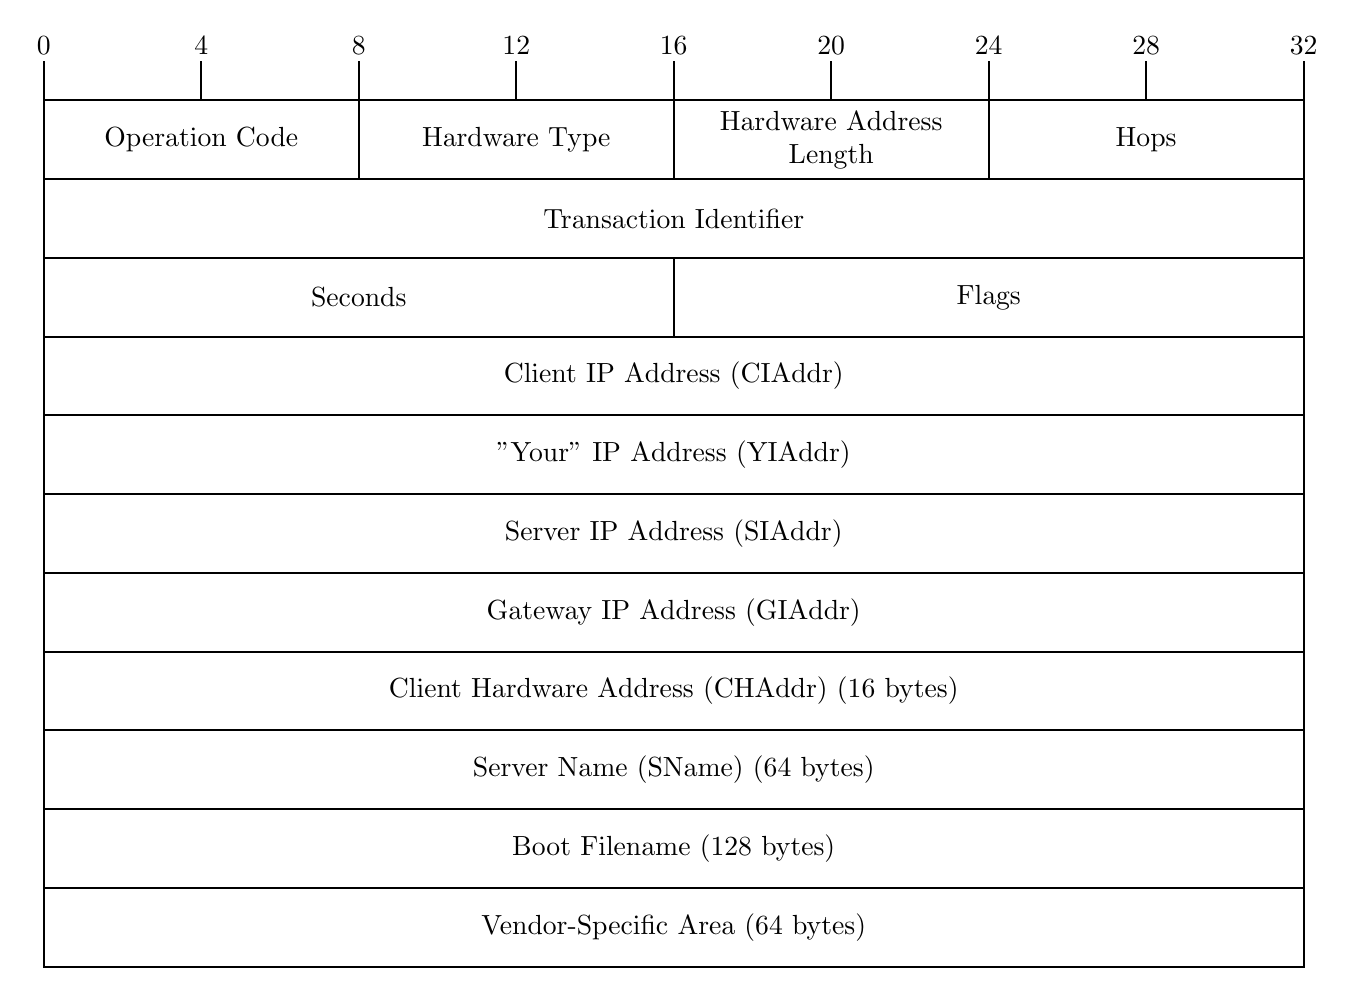
\begin{tikzpicture}
  \draw[line width = 0.75pt, align=center] (0,0) rectangle node{Vendor-Specific Area (64 bytes)} (16,1); 
  \draw[line width = 0.75pt, align=center] (0,1) rectangle node{Boot Filename (128 bytes)} (16,2); 
  \draw[line width = 0.75pt, align=center] (0,2) rectangle node{Server Name (SName) (64 bytes)} (16,3); 
  \draw[line width = 0.75pt, align=center] (0,3) rectangle node{Client Hardware Address (CHAddr) (16 bytes)} (16,4); 
  \draw[line width = 0.75pt, align=center] (0,4) rectangle node{Gateway IP Address (GIAddr)} (16,5); 
  \draw[line width = 0.75pt, align=center] (0,5) rectangle node{Server IP Address (SIAddr)} (16,6); 
  \draw[line width = 0.75pt, align=center] (0,6) rectangle node{"{}Your"{} IP Address (YIAddr)} (16,7); 
  \draw[line width = 0.75pt, align=center] (0,7) rectangle node{Client IP Address (CIAddr)} (16,8); 
  \draw[line width = 0.75pt, align=center] (0,8) rectangle node{Seconds} (8,9); 
  \draw[line width = 0.75pt, align=center] (8,8) rectangle node{Flags} (16,9); 
  \draw[line width = 0.75pt, align=center] (0,9) rectangle node{Transaction Identifier} (16,10); 
  \draw[line width = 0.75pt, align=center] (0,10) rectangle node{Operation Code} (4,11); 
  \draw[line width = 0.75pt, align=center] (4,10) rectangle node{Hardware Type} (8,11); 
  \draw[line width = 0.75pt, align=center] (8,10) rectangle node{Hardware Address\\ Length} (12,11); 
  \draw[line width = 0.75pt, align=center] (12,10) rectangle node{Hops} (16,11); 
  \draw[line width = 0.75pt] (0,11.5) -- node[above=2mm]{0} (0,11);
  \draw[line width = 0.75pt] (2,11.5) -- node[above=2mm]{4} (2,11);
  \draw[line width = 0.75pt] (4,11.5) -- node[above=2mm]{8} (4,11);
  \draw[line width = 0.75pt] (6,11.5) -- node[above=2mm]{12} (6,11);
  \draw[line width = 0.75pt] (8,11.5) -- node[above=2mm]{16} (8,11);
  \draw[line width = 0.75pt] (10,11.5) -- node[above=2mm]{20} (10,11);
  \draw[line width = 0.75pt] (12,11.5) -- node[above=2mm]{24} (12,11);
  \draw[line width = 0.75pt] (14,11.5) -- node[above=2mm]{28} (14,11);
  \draw[line width = 0.75pt] (16,11.5) -- node[above=2mm]{32} (16,11);
\end{tikzpicture}
\caption{BOOTP Message Format}\cite{DHCPr}
\label{fig_BMF}
\end{figure}
--
\begin{description}

\item[Op: ] Gibt den generellen Typ der Nachricht an. Ein Wert von Eins signalisiert eine Anfrage, wobei eine Zwei eine Antwort signalisiert.
\item[HType: ] Spezifiziert die Art der dem Netzwerk zugrunde liegende Hardware. Der Code 1 steht dabei für Ethernet. 
\item[HLen: ] Bezeichnet die Länge der physischen Adressen im Netzwerk. Im Falle von Ethernet Netzwerken sind dies sechs Byte. 
\item[Hops: ] Wird beim Absenden auf Null gesetzt und von jedem {}"Relay Agent"{} um Eins erhöht. 
\item[XID: ] Eine Identifikationsnummer, mit der die Antworten des Servers den Anfragen zugeordnet werden können.
\item[Secs: ] Dieses Feld ist für das Bootstrap Protokoll ungenau definiert und wird oft nicht verwendet. Für DHCP wird es für die Zeit in Sekunden genutzt die vergangen ist, seit der Client damit begonnen hat nach einen neuen {}"Lease"{} zu fragen. 
\item[Flags: ] Acht Bits, die als Flags genutzt werden können. Das erste Bit wird gesetzt, falls die Nachricht als Broadcast gesendet wird, was dem DHCP Server signalisiert, dass dieser über keine gültige IP Adresse verfügt.
\item[CIAddr: ] Steht für "{}Client-IP-Address"{} Der Client schreibt seine eigene IP-Adresse in dieses Feld. Im Falle von DHCP kann dieses nur in den Zuständen BOUND, RENEWING oder REBINDING genutzt werden. In allen anderen Fällen bleibt dieses Feld auf Null.
\item[YIAddr: ] Abkürzung für "Your IP Address". Wird vom Server gesetzt um den Client eine IP-Adresse zuzuweisen. 
\item[SIAddr: ] Der Server gibt hier die Adresse des Servers an, dem der Client seine nächste Anfrage schicken soll. 
\item[GIAddr: ] Wird nur im {}"Bootstrap Protocol"{} für die Kommunikation zwischen Client und Server verwendet, wenn diese nicht im selben Netzwerk oder Subnet liegen. Wird im DHCP nicht dafür verwendet, das Standardgateway anzugeben. 
\item[CHAddr: ] Hardware Adresse des Clients. Bei Nutzung von Ethernet die Mac-Adresse. 
\item[SName: ] Der DHCP-Server kann hier optional seinen Namen angeben. Alternativ kann dieses Feld durch die "{}Option overload"{} Funktion auch für weitere Optionen genutzt werden.
\item[File: ] Kann genutzt werden, um bei einem DHCPDISCOVER oder OFFER eine Bootdatei anzugeben. 
\item[Options: ] Für das Bootstrap-Protokoll gibt es eine große Menge an Optionen, einige davon werden exklusiv für DHCP genutzt. \\
Die Anzahl und Art der verwendeten Optionen ist variabel. Der Aufbau von diesen folgt jedoch einem definierten Format. Die ersten acht Bit eines Optionsblocks enthalten den Code der Option, weitere acht Bit geben die Länge des folgenden Datenfeldes an. Das Optionfeld beginnt im Falle von DHCP mit der {}"Magic Number"{} 99.130.83.99. Nur dann können die exklusiven DHCP-Optionen genutzt werden.\cite{DHCPr}
Dazu gehören:
\begin{description}
	\item[Requested IP Address:] Diese Option kann während eines DHCP-Discovers gesetzt werden, um die Verfügbarkeit einer bestimmten IP-Adresse anzufragen.\\
	Code: 50; Länge: 4 Byte;
	 
	\item[IPAddress Lease Time:] Kann in einer DHCP-Request oder DHCP-Offer Nachricht gesetzt werden. Der Client kann dabei eine bestimmte Lease-Time in Sekunden angeben.\\
	Code: 51; Länge: 4 Byte;
	
	\item[Option Overload:] Diese Option signalisiert, dass Option Overload genutzt wird. Das bedeutet, dass weitere Optionen anstelle der Felder SNAME oder FILE geschrieben werden. \\
	Code: 52; Länge: 1 Byte;
	Es gibt drei mögliche Werte, die geschrieben werden können: 
	\begin{itemize}
		\item 1: Optionen stehen im File-Feld. 
		\item 2: Optionen stehen im SNAME-Feld.
		\item 3: Optionen stehen in beiden Feldern.
	\end{itemize}
	
	\item[DHCP Message Type] Dieses Feld ist bei DHCP-Nachrichten immer vorhanden und gibt die Art der DHCP-Nachricht an. \\
	Code: 53; Länge: 1 Byte;
	\begin{itemize}
		\item 1: DHCPDISCOVER
		\item 2: DHCPOFFER
		\item 3: DHCPREQUEST
		\item 4: DHCPDECLINE
		\item 5: DHCPACK
		\item 6. DHCPNAK
		\item 7: DHCPRELEASE
		\item 8: DHCPINFORM		
		
	\end{itemize}
	
	\item[Server Identifier:] Die Option kann von einem Client bei einer DHCP-Request gesetzt werden, um bei Unicast-Nachrichten die Adresse von einem bestimmten Server anzugeben. Ein DHCP-Server kann dieses Feld setzten, damit ein Client mehrere DHCP-Offer unterscheiden kann. \\
	Code: 54; Länge: 4 Byte;
	
	
	\item[Parameter Request List:] Es kann eine Liste von Parametern übergeben werden um die Werte von diesen bei einem Server anzufragen. Dazu kann eine beliebig lange Folge aus DHCP/Bootstrap Optionscodes genutzt werden.\\
	Code: 55; Länge: n Byte;	
\end{description}
\end{description}
\subsection{Ablauf}

Zu Beginn eines DHCP-Vorgangs, wenn zum Beispiel ein Client hochgefahren wird, verfügt dieser weder über eine IP-Adresse, noch über andere Information die Netzwerktopologie betreffend. Als Erstes sendet der Client ein Discover-Paket. Dafür wird der Operationscode auf 1 gesetzt um ein Request-Paket zu signalisieren, die MAC-Adresse wird für die physische Client Adresse verwendet, das Broadcast-Flag wird gesetzt und der DHCP-Message-Type wird auf Discover gesetzt. Aus diesem DHCP-Paket wird ein UDP-Paket erzeugt, mit dem Quellport  68 und dem Zielport 67. Die Nachricht wird als Broadcast gesendet. \\
Auf diese Anfrage können einer oder mehrere DHCP-Server antworten. Wenn kein bestimmter Server in der DISCOVER-Nachricht spezifiziert wurde, schicken alle Server in dem jeweiligen Netzwerk ein "{}OFFER". Diese Nachricht wird ebenfalls als Broadcast gesendet, da der Client noch keine eigene IP zugewiesen hat. Das OFFER enhält einen Vorschlag mit einer IP-Adresse in dem Feld "Your-IP-Address". Anhand der "Transaction ID"{} und dem Feld CHADDR kann der Client die Offer eindeutig seiner Anfrage zuordnen. \\
Der Client antwortet auf das "{}OFFER"{} mit einer {}"REQUEST"{}-Nachricht. Dafür wird die Option "Requested-IP-Address"{} gesetzt. \\
Auf das Request antwortet der Server wiederum mit einem ACK zu Bestätigung. Wenn der Client die Bestätigung erhält, prüft dieser, ob die IP-Adresse schon genutzt wird, in dem er eine ARP-Request für diese startet. Wird diese beantwortet, ist die Adresse schon in Benutzung. Ist dies nicht der Fall, übernimmt der Client die Adresse. 
Die ACK Nachricht enthält die Lease-Zeit, welche angibt, wie lange eine IP gültig ist. 
Nachdem die Hälfte der Lease-Zeit abgelaufen ist, sendet der Client eine weitere REQUEST-Nachricht. Da er zu diesem Zeitpunkt noch über eine gültige IP-Adresse verfügt, sendet er die Nachricht nicht als Broadcast, sondern als Unicast direkt an den DHCP-Server, von dem er die IP zugewiesen bekommen hat. In dem Fall, dass er auf den Request keine Antwort bekommen hat, startet er nach Ablauf der Lease Zeit mit einem DISCOVER.\\
Während dieses Vorgangs können neben der IP auch noch andere Informationen abgefragt werden. Wie beispielsweise die Adressen von DNS- und Zeitservern.\cite{DHCPr}




\chapter{AMIDAR Prozessor}
Bei der Klasse der AMIDAR-Prozessoren handelt es sich um rekonfigurierbare Systeme, die zur Laufzeit an die Anwendung angepasst werden können. Sie bestehen jeweils aus mehreren {}"Function Units"{}, die über ein Token- und ein Datennetzwerk verbunden sind. Ein Token stellt dabei eine Mikroinstruktion dar. Diese werden durch die Tokenmaschine aus den Prozessor-Instruktionen generiert. Dazu kommen FUs für Framestack, Heap, ALUs und Hardwarebeschleuniger. Bei den in Hardware implementierten Prototypen des Fachgebiets Rechnersysteme wird Java-Bytecode eingesetzt.

\begin{figure}[h]
\centering
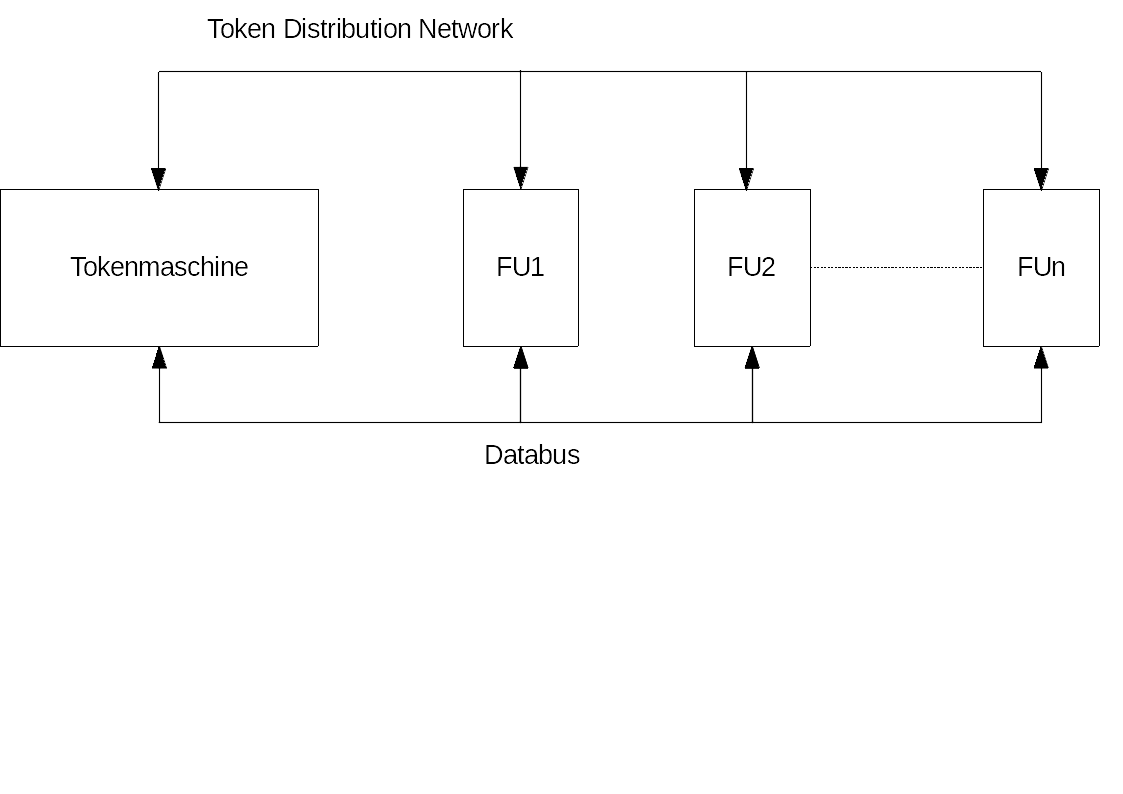
\includegraphics[width=0.75\textwidth]{Graphics/AMIDAR.png}
\caption{AMIDAR Aufbau}
\end{figure}
